%!TEX TS-program = xelatex
%!TEX encoding = UTF-8 Unicode

\documentclass[12pt]{extarticle}
% extarticle is like article but can handle 8pt, 9pt, 10pt, 11pt, 12pt, 14pt, 17pt, and 20pt text

\def \ititle {Origins of Mind}

\def \isubtitle {Lecture 02}

\def \iauthor {Stephen A. Butterfill}
\def \iemail{s.butterfill@warwick.ac.uk}
\date{}

%for strikethrough
\usepackage[normalem]{ulem}

\input{$HOME/Documents/submissions/preamble_steve_handout}

%\bibpunct{}{}{,}{s}{}{,}  %use superscript TICS style bib
%remove hanging indent for TICS style bib
%TODO doesnt work
\setlength{\bibhang}{0em}
%\setlength{\bibsep}{0.5em}


%itemize bullet should be dash
\renewcommand{\labelitemi}{$-$}

\begin{document}

\begin{multicols}{3}

\setlength\footnotesep{1em}


\bibliographystyle{newapa} %apalike

%\maketitle
%\tableofcontents




%---------------
%--- start paste






\def \ititle {Lecture 04}

\begin{center}

{\Large

\textbf{\ititle}

}



\iemail %

\end{center}

\section{Background}

Knowledge of objects depends on abilities to (i) segment objects, (ii) represent them as
persisting and (iii) track their interactions.

\emph{Question 1}  When do humans come to meet the three requirements on knowledge of objects?

\emph{Discovery 1} Infants manfiest all three abilities from around four months of age or earlier.

\emph{Question 2}  How do humans come to meet the three requirements on knowledge of objects?

\emph{Discovery 2} Although abilities to segment objects, to represent them as persisting through
occlusion and to track their causal interactions are conceptually distinct, they
are all characterised by the Principles of Object Perception and they may all be
consequences of a single mechanism.

\emph{Question 3} What is the relation between the model specified by the Principles of Object
Perception and the infants?

\textit{The simple view}
The principles of object perception are things that we know or believe,
and we generate expectations from these principles by a process of inference.

The \emph{Core Knowledge View}
The principles of object perception are not
knowledge, but they are core knowledge. And we generate expectations from
these principles by a process of inference.

\emph{Discovery 3} The Simple View generates systematically false predictions.
(And the Core Knowledge View generates no relevant predictions by itself.)

\emph{Question 4} What is the relation between adults’ and infants’ abilities concerning physical
objects and their causal interactions?



\section{The CLSTX Hypothesis: Object Indexes Underpin Infants’ Abilities}

Leslie et al say an object index is ‘a mental token that functions as a pointer to an
object’ \citep[p.\ 11]{Leslie:1998zk}

‘Pylyshyn’s FINST model: you have four or five indexes which can be attached to objects;
it’s a bit like having your fingers on an object: you might not know anything about the
object, but you can say where it is relative to the other objects you’re fingering.
(ms. 19-20)’ \citep{Scholl:1999mi}

Object indexes ...
\begin{itemize}
\item guide ongoing action (e.g.~visual tracking, reaching)
\item influence how attention is allocated
\citep{flombaum:2008_attentional}
\item can be assigned in ways incompatible with beliefs and knowledge \citep[e.g.][]{Mitroff:2004pc, mitroff:2007_space}
\item have behavioural  and neural markers, in adults and infants   \citep{richardson:2004_multimodal,kaufman:2005_oscillatory}.
\item are subject to signature limits \citep[pp.~83--87]{carey:2009_origin}
\item sometimes survive occlusion \citep{flombaum:2006_temporal}
\end{itemize}

The \emph{object-specific preview benefit} is the reduction in time needed to identify that a
letter (or other feature) matches a target presented earlier when the letter and target both
appear on the same object rather than on different objects.


\emph{The CLSTX conjecture}
Infants’ abilities concerning physical objects are
characterised by the Principles of Object Perception because infants’ abilities
are a consequence of the operations of a system of object indexes
\citep{Leslie:1998zk,Scholl:1999mi,Carey:2001ue,scholl:2007_objecta}.

A \emph{{signature limit} of a system} is a pattern of behaviour the system exhibits which is
both defective given what the system is for and peculiar to that system.



\section{Core Knowledge vs Object Indexes}

Consider the conjecture that infants’ abilities concerning physical objects are
characterised by the Principles of Object Perception because infants’ abilities
are a consequence of the operations of a system of object indexes.
If this conjecture is true, should we reject the claim that infants have a core
system for physical objects?
Or does having a system of object indexes whose operations are characterised by the Principles of
Object Perception amount to having core knowledge of those principles?

\emph{Outstanding problem}
Since having core knowledge of objects does not imply having knowledge knowledge of objects, how
can the emergence in development of knowledge of simple facts about particular physical objects be
explained?
What is the role of core knowledge of objects, and what other factors might be involved?



\section{Phenomenal Expectations Connect Object Indexes to Looking Behaviours}

How could the operations of object indexes explain purposive actions like looking longer at one
thing than another?

First idea: the operations of object indexes give rise to corresponding beliefs.
Objection: if four- and five-month-olds had such beliefs they should search for occluded objects,
which they do not \citep[e.g.][]{Shinskey:2001fk,moore:2008_factors}.
And anyway, object indexes do not always give rise to beliefs even in adults \citep{Mitroff:2004pc}.

Second idea: phenomenal expectations ...

\emph{Phenomenal Expectations}
are aspects of the overall phenomenal character of experiences which their subjects take to be
informative about things that are only distantly related (if at all) to the things that those
experiences intentionally relate the subject to.

Phenomenal expectations can be thought of as sensations in approximately Reid’s sense: they are
monadic properties of events, specifically perceptual experiences, which are individuated by their
normal causes
and which alter the overall phenomenal character of those experiences in ways not determined by the
experiences’ contents
(so two perceptual experiences can have the same content but distinct sensational properties).

Phenomenal expectations are signs:
they can lead to beliefs only via associations or further beliefs
(\citealp[Essay~II, Chap.~16, p.~228]{Reid:1785cj};
\citealp[Chap.~VI sect.~III, pp.~164–5]{Reid:1785nz}).

\section{Development is Rediscovery}
How do you get from core knowledge to knowledge proper?

\emph{The Assumption of Representational Connections}: the transition involves operations on the contents of core knowledge states, which transform them into (components of) the contents of knowledge states.

Most proposals rely on this assumption, including:
(i) Spelke’s suggestion that mature understanding of objects derives from core knowledge by virtue of core knowledge representations being assembled (\citeyear{Spelke:2000nf}); (ii) claims by Leslie and others that modules provide conceptual identifications of their inputs \citep{Leslie:1988ct}; (iii) Karmiloff-Smith’s representational re-description (\citeyear{Karmiloff-Smith:1992lv}); and (iv) Mandler’s claim that ‘the earliest conceptual functioning consists of a redescription of perceptual structure’ (\citeyear{Mandler:1992vn}).
%\begin{itemize}
%\item assembling core knowledge from different domains \citep{Spelke:2000nf}
%\item modules provide conceptual identifications of their inputs
%\citep{Leslie:1988ct}
%\item representational re-description
%\citep{Karmiloff-Smith:1992lv}
%\item ‘the earliest conceptual functioning consists of a redescription of perceptual structure’ \citep{Mandler:1992vn}
%\end{itemize}

If object indexes influence actions only via phenomenal expectations, the Assumption of Representational Connections is wrong.

\emph{Alternative assumption}: the transition depends only on the effects of core knowledge states on behaviour, attention, and sensation.

Development is rediscovery: the emergence of knowledge involves rediscovering information already encoded as core knowledge.



\section{Syntax / Innateness}

Is the syntactic structure of ‘the red ball’ (a) flat or (b) hierachical?

\begin{center}

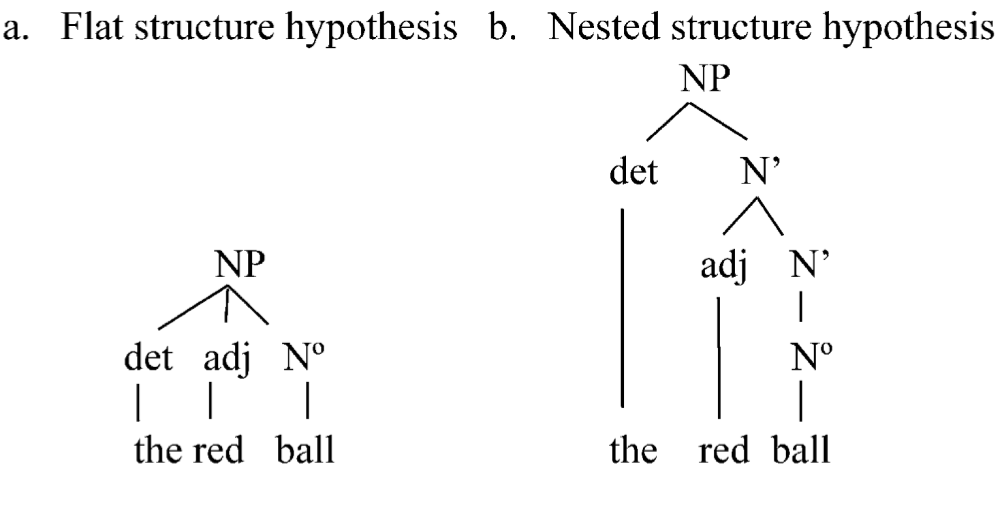
\includegraphics[scale=0.25]{../www.slides/src/raw/img/lidz_2003_fig0.neg.png}

\end{center}

\begin{center} from \citealp{lidz:2003_what} \end{center}

\begin{enumerate}



\item ‘red ball’ is a constituent on (b) but not on (a)


\item anaphoric pronouns can only refer to constituents



                \item In the sentence ‘I’ll play with this red ball and you can play with that one.’, the word ‘one’ is an anaphoric prononun that refers to ‘red ball’ (not just ball).
                \citep{lidz:2003_what,lidz:2004_reaffirming}.




\end{enumerate}

‘The assumption in the preferential looking task is that infants prefer to look at an image that matches the linguistic stimulus, if one is available’ \citep{lidz:2003_what}.

\subsection{Poverty of stimulus arguments}

How do poverty of stimulus arguments work? See \citet{pullum:2002_empirical}.

\begin{enumerate}

\item

Human infants acquire X.

\item

To acquire X by data-driven learning you'd need this  Crucial Evidence.

\item

But infants lack this Crucial Evidence for X.

\item

So human infants do not acquire X by data-driven learning.

\item

But all acquisition is either data-driven or innately-primed learning.

\item

So human infants acquire X by innately-primed learning .

\end{enumerate}

‘the APS [argument from the poverty of stimulus] still awaits even a single good supporting example’
\citep[p.\ 47]{pullum:2002_empirical}


    




%--- end paste
%---------------

\footnotesize
\bibliography{$HOME/endnote/phd_biblio}

\end{multicols}

\end{document}
